% ============================================================
%  NITK SURATHKAL — IT 351 Human Computer Interaction
%  VI Semester B.Tech.(IT) Project Report
%  Health Record Management System
% ============================================================
\documentclass[12pt,a4paper]{report}

% ── Packages ─────────────────────────────────────────────────
\usepackage[left=1in,right=1in,top=1in,bottom=1in]{geometry}
\usepackage{times}           % Times New Roman
\usepackage{fontenc}
\usepackage{inputenc}
\usepackage{graphicx}
\graphicspath{{diagrams/}}
% NOTE: pdflatex cannot include .svg directly.
% Convert SVGs to PDF first using Inkscape (run once):
%   inkscape --export-type=pdf diagrams/fig1_system_architecture.svg
%   inkscape --export-type=pdf diagrams/fig2_auth_flow.svg
%   inkscape --export-type=pdf diagrams/fig3_record_lifecycle.svg
%   inkscape --export-type=pdf diagrams/fig4_er_diagram.svg
%   inkscape --export-type=pdf diagrams/fig5_frontend_structure.svg
% Or use: for %f in (diagrams\*.svg) do inkscape --export-type=pdf "%f"
% The \includegraphics calls below will then find the .pdf files automatically.
\usepackage{booktabs}
\usepackage{longtable}
\usepackage{array}
\usepackage{setspace}
\usepackage{titlesec}
\usepackage{tocloft}
\usepackage{hyperref}
\usepackage{caption}
\usepackage{float}
\usepackage{enumitem}
\usepackage{xcolor}
\usepackage{listings}
\usepackage{amsmath}
\usepackage{fancyhdr}
\usepackage{pdfpages}
\usepackage{microtype}
\usepackage{url}
\usepackage{parskip}

% ── No headers / footers; page number at bottom middle ───────
\pagestyle{plain}
\fancyhf{}

% ── Paragraph spacing (1.5 line spacing for body) ────────────
\setstretch{1.5}

% ── Caption formatting ───────────────────────────────────────
\captionsetup{font={bf,small},labelsep=period,justification=centering}
\captionsetup[table]{position=above}
\captionsetup[figure]{position=below}

% ── Chapter / section heading format ─────────────────────────
%  Main Heading  : Times 16 pt, bold, centred, numbered
\titleformat{\chapter}[block]
  {\fontsize{16}{20}\selectfont\bfseries\centering}  % format
  {\thechapter.}                                      % label
  {0.5em}                                             % sep
  {}                                                  % before-code
  [\vspace{24pt}]                                    % after-code (2 blank lines ≈ 24 pt)

%  Sub-heading level 1 : Times 14 pt, bold, italic, left
\titleformat{\section}
  {\fontsize{14}{18}\selectfont\bfseries\itshape}
  {\thesection}
  {0.5em}{}

%  Sub-heading level 2 : Times 12 pt, bold, left
\titleformat{\subsection}
  {\fontsize{12}{16}\selectfont\bfseries}
  {\thesubsection}
  {0.5em}{}

% ── Hyperlink colours ─────────────────────────────────────────
\hypersetup{
  colorlinks=true,
  linkcolor=black,
  urlcolor=blue,
  citecolor=black
}

% ── Code listings style ───────────────────────────────────────
\lstset{
  basicstyle=\ttfamily\small,
  breaklines=true,
  frame=single,
  captionpos=b,
  numbers=left,
  numberstyle=\tiny
}

% ─────────────────────────────────────────────────────────────
\begin{document}

% ============================================================
%  FRONT MATTER  (no page numbers)
% ============================================================
\pagenumbering{gobble}

% ────────────────────────────────────────────────────────────
%  1. COVER PAGE
% ────────────────────────────────────────────────────────────
\begin{titlepage}
\centering
\vspace*{0.5cm}
{\Large\bfseries DEPARTMENT OF INFORMATION TECHNOLOGY\\[4pt]
NATIONAL INSTITUTE OF TECHNOLOGY KARNATAKA, SURATHKAL\\[2pt]
Mangaluru -- 575025}\\[1.5cm]

{\large\bfseries IT 351 -- Human Computer Interaction}\\[0.3cm]
{\large (VI Semester B.Tech. -- Jan -- May 2026 Session)}\\[2cm]

{\Huge\bfseries Health Record Management System}\\[2cm]

{\large\bfseries Submitted by:}\\[0.5cm]
{\large
\begin{tabular}{ll}
Student Name & : \textit{[Author Name(s)]}\\[4pt]
Roll Number  & : \textit{[Roll Number(s)]}\\[4pt]
\end{tabular}}\\[2cm]

{\large\bfseries Under the Guidance of:}\\[0.5cm]
{\large Dr.\ Deepa C}\\[0.2cm]
{\large Course Instructor, Department of Information Technology}\\[3cm]

\includegraphics[width=3cm]{nitk_logo.png}   % Replace with actual logo path

\vfill
{\large April 2026}
\end{titlepage}

% ────────────────────────────────────────────────────────────
%  2. DECLARATION
% ────────────────────────────────────────────────────────────
\chapter*{Declaration by the Student}
\addcontentsline{toc}{chapter}{Declaration by the Student}

We, the undersigned, hereby declare that the project report titled \textbf{``Health Record Management System''}, submitted to the Department of Information Technology, National Institute of Technology Karnataka, Surathkal, in partial fulfilment of the requirements for the course IT 351 — Human Computer Interaction (VI Semester B.Tech., Jan -- May 2026 Session), is an original work carried out by us. The project report has not been submitted elsewhere for the award of any degree or diploma.

All sources of information and references used in the preparation of this report have been duly acknowledged.

\vspace{2cm}
\noindent
\begin{tabular}{ll}
Name    & : \rule{6cm}{0.5pt}\\[12pt]
Roll No & : \rule{6cm}{0.5pt}\\[12pt]
Date    & : \rule{6cm}{0.5pt}\\[12pt]
Place   & : Surathkal, Karnataka
\end{tabular}

\vspace{1.5cm}
\noindent\textbf{Signature:}~~\rule{5cm}{0.5pt}

% ────────────────────────────────────────────────────────────
%  3. CERTIFICATE
% ────────────────────────────────────────────────────────────
\chapter*{Certificate}
\addcontentsline{toc}{chapter}{Certificate}

This is to certify that the project report entitled \textbf{``Health Record Management System''} submitted by \textit{[Student Name(s)]} (Roll No.\ \textit{[Roll Number(s)]}) is a record of bonafide work carried out by them under my guidance in the VI Semester of B.Tech.\ (Information Technology) for the course IT 351 — Human Computer Interaction (Jan -- May 2026 Session) at the National Institute of Technology Karnataka, Surathkal.

\vspace{2.5cm}
\noindent
\begin{tabular}{ll}
\textbf{Dr.\ Deepa C} & \\[4pt]
Course Instructor & \\[4pt]
Department of Information Technology & \\[4pt]
NIT Karnataka, Surathkal & \\[12pt]
Date: \rule{4cm}{0.5pt} &
\end{tabular}

% ────────────────────────────────────────────────────────────
%  4. ACKNOWLEDGEMENTS
% ────────────────────────────────────────────────────────────
\chapter*{Acknowledgements}
\addcontentsline{toc}{chapter}{Acknowledgements}

We would like to express our sincere gratitude to \textbf{Dr.\ Deepa C}, Course Instructor, Department of Information Technology, NIT Karnataka, Surathkal, for her invaluable guidance, encouragement, and insightful feedback throughout the development of this project.

We are thankful to the Department of Information Technology, NITK Surathkal, for providing the necessary infrastructure and resources. We also acknowledge the open-source communities behind React, Node.js, Express, MongoDB, and Tailwind CSS whose tools formed the backbone of this project.

Finally, we thank our friends and families for their continuous support.

% ────────────────────────────────────────────────────────────
%  5. ABSTRACT
% ────────────────────────────────────────────────────────────
\chapter*{Abstract}
\addcontentsline{toc}{chapter}{Abstract}

The \textbf{Health Record Management System (HRMS)} is a comprehensive, role-based web application designed to centralise the management of patient health records across multiple hospitals and healthcare stakeholders. In the current healthcare ecosystem, patient medical information is often siloed within individual hospital databases, forcing patients to carry physical documents and making it difficult for healthcare providers to access complete clinical histories at the point of care. This fragmentation leads to diagnostic errors, redundant investigations, and compromised patient outcomes.

This project addresses these challenges by delivering a unified digital platform that serves five distinct user roles: \textit{Patient}, \textit{Doctor}, \textit{Nurse}, \textit{Hospital}, and \textit{Administrator}. Patients can view their complete consolidated medical history, manage prescriptions and diagnostic reports, monitor health analytics derived from real-world visits, and integrate wearable device data (smartwatch metrics such as heart rate, steps, SpO\textsubscript{2}, and sleep hours). Doctors can access authorised patient records, create prescriptions, upload diagnostic documents, and annotate records collaboratively. Nurses can update vital signs, manage custom clinical fields, and handle test assignments. Hospital administrators can manage affiliated staff, approved test types, and audit logs. System administrators can oversee hospital registrations and user management across the entire platform.

From a Human--Computer Interaction (HCI) perspective, this project prioritises accessibility, usability, and inclusive design. The system implements a comprehensive accessibility framework including dyslexia-friendly typography, keyboard-only navigation, text-size scaling, target-boost mode for motor-impaired users, form assist mode, and accessible chart rendering. The frontend follows the \textit{Governance Terminal} design language — a dark-mode-first, emerald-accented UI built in React with Tailwind CSS, emphasising clarity, information hierarchy, and responsive layouts across desktop and mobile viewports.

The backend is implemented as a RESTful API using Node.js and Express.js, with MongoDB as the persistent data store. AI-assisted document parsing is integrated via a configurable provider (Ollama or Google Gemini) to extract structured information from uploaded medical PDFs. JSON Web Token (JWT) authentication enforces role-based access to all API endpoints. The system is designed to be modular, extensible, and secure, meeting modern standards for web-based health information systems.

\textbf{Keywords:} Health Record Management, Electronic Health Records (EHR), Role-Based Access Control, Human--Computer Interaction, Accessibility, React, Node.js, MongoDB, REST API.

% ────────────────────────────────────────────────────────────
%  TABLE OF CONTENTS
% ────────────────────────────────────────────────────────────
\tableofcontents

% ────────────────────────────────────────────────────────────
%  LIST OF FIGURES
% ────────────────────────────────────────────────────────────
\listoffigures

% ────────────────────────────────────────────────────────────
%  LIST OF TABLES
% ────────────────────────────────────────────────────────────
\listoftables

% ============================================================
%  MAIN MATTER  (Arabic page numbers from Chapter 1)
% ============================================================
\pagenumbering{arabic}
\setcounter{page}{1}

% ============================================================
%  CHAPTER 1 — INTRODUCTION
% ============================================================
\chapter{Introduction}

Healthcare is one of the most data-intensive domains in the modern world. A typical patient produces dozens of clinical data points across every hospital visit: diagnoses, prescriptions, diagnostic reports, vital signs, and follow-up instructions. When this information is locked within a single institution's local system, the patient is expected to act as their own health record carrier — remembering dosages, bringing physical files, and re-narrating their clinical history to every new provider they visit.

Electronic Health Record (EHR) systems have long been proposed as the solution to this fragmentation. However, nationwide or cross-institutional EHR adoption remains limited in many regions, particularly in developing healthcare economies. Patients who visit multiple hospitals — or who shift residence and change providers — are disproportionately affected. In emergency situations, the absence of complete medical history (allergies, chronic conditions, current medications) can be life-threatening.

The \textbf{Health Record Management System (HRMS)} presented in this report is a full-stack web application built as part of the IT 351 Human--Computer Interaction (HCI) course at NIT Karnataka, Surathkal. It demonstrates how modern HCI principles — role-tailored interfaces, accessibility features, responsive design, and real-time feedback mechanisms — can be applied to solve a pressing societal problem in healthcare.

The system is architected around five roles, each with a purpose-built dashboard: \textit{Patient}, \textit{Doctor}, \textit{Nurse}, \textit{Hospital}, and \textit{Admin}. The solution is built on a MERN stack (MongoDB, Express.js, React, Node.js) with a Vite-powered frontend and a RESTful backend. AI-powered document parsing enables automatic extraction of structured data from uploaded medical PDFs.

\section{Challenges}

\subsection{1.1.1 Fragmented Patient Data}
Medical records in India and many developing nations are predominantly paper-based or stored in institution-specific software with no interoperability. When patients switch hospitals, their history is unavailable, leading to redundant tests and incomplete diagnoses.

\subsection{1.1.2 Multi-Stakeholder Complexity}
A single patient encounter involves multiple roles: doctors, nurses, administrative staff, and hospital management. Designing a unified platform that respects role-based access control without compromising usability presented a significant design and engineering challenge.

\subsection{1.1.3 Accessibility and Inclusive Design}
Healthcare platforms have a moral responsibility to be accessible to users with disabilities. Many existing portals lack support for dyslexia-friendly typography, keyboard navigation, or scalable text. Incorporating a comprehensive accessibility framework without disrupting the primary visual design is non-trivial.

\subsection{1.1.4 Secure Data Handling}
Medical data is among the most sensitive personal data categories. Ensuring end-to-end security — HTTPS-ready APIs, JWT-based authentication, bcrypt password hashing, and role-enforced API routes — while maintaining performance was a key engineering challenge.

\subsection{1.1.5 AI Integration for Document Parsing}
Uploaded diagnostic PDFs are diverse in format and style. Integrating an AI pipeline to extract structured clinical data (diagnosis, medications, health metrics, report dates) from heterogeneous documents required careful prompt engineering and a resilient extraction architecture.

\section{Motivation for the Work}

The motivation for building HRMS stems from three intersecting needs:

\begin{enumerate}[leftmargin=2cm]
    \item \textbf{Societal Need}: Centralised patient health records reduce diagnostic errors, prevent duplicate testing, and empower patients with ownership of their own health data.
    \item \textbf{HCI Education}: Building a multi-role, accessible healthcare interface provides a rich applied context for practising and demonstrating HCI principles including user-centred design, accessibility (WCAG), usability heuristics, and responsive UI engineering.
    \item \textbf{Technical Relevance}: The MERN stack combined with AI-assisted document parsing and wearable device integration represents a contemporary, industry-relevant technology combination, offering practical exposure to full-stack engineering patterns.
\end{enumerate}

The project is grounded in the belief that good interface design in healthcare is not simply aesthetic — it is a patient-safety concern.

% ============================================================
%  CHAPTER 2 — LITERATURE SURVEY
% ============================================================
\chapter{Literature Survey}

\section{Introduction to Literature Survey}

The domain of Electronic Health Records (EHR) and health information management has been extensively studied from both technical and HCI perspectives. This chapter surveys the relevant literature on centralised health record systems, role-based access in healthcare, web-based EHR platforms, and accessibility considerations in digital health applications. The review informs the design decisions made in the HRMS project.

\section{Related Work}

\subsection{2.2.1 Electronic Health Record Systems}
Berner et al.\ (2005) conducted a comprehensive survey of EHR systems and identified data fragmentation and lack of interoperability as the primary barriers to adoption \cite{berner2005}. The HL7 FHIR (Fast Healthcare Interoperability Resources) standard, introduced by the HL7 organisation, has since emerged as the leading specification for exchanging healthcare data electronically \cite{hl7fhir}.

Jha et al.\ (2009) studied EHR adoption across US hospitals and found that fewer than 2\% had a fully functional EHR system at the time, citing cost, complexity, and workflow disruption as barriers \cite{jha2009}. This study reinforces the need for lightweight, web-native EHR platforms that are accessible to smaller and non-academic hospitals.

\subsection{2.2.2 Role-Based Access Control in Healthcare}
Ferraiolo et al.\ (2001) formalised Role-Based Access Control (RBAC) as a standard access policy model, showing that roles are the most natural unit of access for organisational information systems \cite{ferraiolo2001}. In healthcare, patient data must be accessible to treating doctors but restricted from unaffiliated staff. This directly motivates the five-role model implemented in HRMS.

\subsection{2.2.3 Web-Based Patient Portals}
Roblin et al.\ (2009) evaluated the Kaiser Permanente patient portal and found that patients who accessed their records online had higher rates of preventive care and better chronic disease management \cite{roblin2009}. This supports the design decision to give patients full read access to their medical history, prescriptions, and analytics in HRMS.

\subsection{2.2.4 HCI and Usability in Health Applications}
Middleton et al.\ (2013) observed that poor usability of EHR interfaces was a leading contributor to physician burnout and clinical error \cite{middleton2013}. They recommended adherence to Nielsen's usability heuristics — particularly visibility of system status, error prevention, and recognition over recall — as design goals. HRMS addresses these through toast notifications, confirmation dialogs, and inline form validation.

\subsection{2.2.5 Accessibility in Digital Health}
Lazar et al.\ (2015) emphasised that health IT systems must be accessible to users with motor, visual, and cognitive disabilities, noting that this population disproportionately relies on digital health services \cite{lazar2015}. The HRMS accessibility framework (dyslexia mode, keyboard navigation, target boost, text scaling) was directly motivated by these findings.

\subsection{2.2.6 AI-Assisted Medical Document Analysis}
Rajpurkar et al.\ (2022) demonstrated that large language models can extract structured clinical information from unstructured medical reports with accuracy comparable to human annotators when given domain-specific prompts \cite{rajpurkar2022}. This finding motivated the inclusion of an LLM-based document parsing pipeline (Ollama/Gemini) in HRMS to automatically extract diagnosis, medications, and metrics from uploaded PDFs.

\subsection{2.2.7 Wearable Device Integration}
Piwek et al.\ (2016) reviewed the use of consumer wearables in healthcare and concluded that heart rate, step count, and sleep data from devices such as Fitbit and Apple Watch are clinically meaningful when provided alongside traditional medical records \cite{piwek2016}. HRMS integrates a Smartwatch Insights module that fetches and visualises these metrics.

\section{Outcome of Literature Review}

The literature review reveals a clear consensus: centralised, role-stratified, usable, and accessible EHR platforms reduce clinical errors and improve patient outcomes. Key design principles extracted from the literature and applied in HRMS are:

\begin{itemize}
    \item Role-Based Access Control (RBAC) as the access policy model
    \item Patient portal with full read access to records and analytics
    \item Adherence to Nielsen's usability heuristics in UI design
    \item WCAG-aligned accessibility features
    \item AI-assisted extraction for unstructured medical documents
    \item Wearable device data integration for longitudinal health monitoring
\end{itemize}

\section{Problem Statement}

Patients visiting multiple hospitals in India and similar healthcare systems bear the burden of maintaining, carrying, and re-presenting their medical records at every consultation. Healthcare providers lack immediate access to a patient's complete history, leading to redundant investigations, medication conflicts, and suboptimal care. Existing hospital management software is siloed, non-interoperable, and often inaccessible to users with disabilities. There is a need for a secure, interoperable, role-based, and inclusive web platform that centralises patient health records and provides HCI-centric interfaces tailored to each stakeholder.

\section{Research Objectives}

\begin{enumerate}[leftmargin=2cm]
    \item To design and implement a centralised health record management system serving five user roles (Patient, Doctor, Nurse, Hospital, Admin) with role-specific dashboards.
    \item To enforce role-based access control at both the API layer and the frontend route level.
    \item To integrate an AI-powered pipeline for automatic extraction of structured clinical data from uploaded medical PDF documents.
    \item To implement a comprehensive accessibility framework compliant with WCAG 2.1 AA guidelines.
    \item To provide patients with real-time health analytics derived from their visit history and smartwatch data.
    \item To apply HCI principles — including responsive design, micro-animations, inline feedback, and consistent design language — across all modules.
\end{enumerate}

% ============================================================
%  CHAPTER 3 — METHODOLOGY AND FRAMEWORK
% ============================================================
\chapter{Methodology and Framework}

\section{Block Diagram and Flowchart}

\subsection{3.1.1 System Architecture}

The HRMS follows a three-tier client-server architecture:

\begin{itemize}
    \item \textbf{Presentation Tier}: React (Vite) SPA with Tailwind CSS
    \item \textbf{Application Tier}: Node.js + Express.js RESTful API
    \item \textbf{Data Tier}: MongoDB (Mongoose ODM)
\end{itemize}

\begin{figure}[H]
\centering
% Replace with actual architecture diagram image
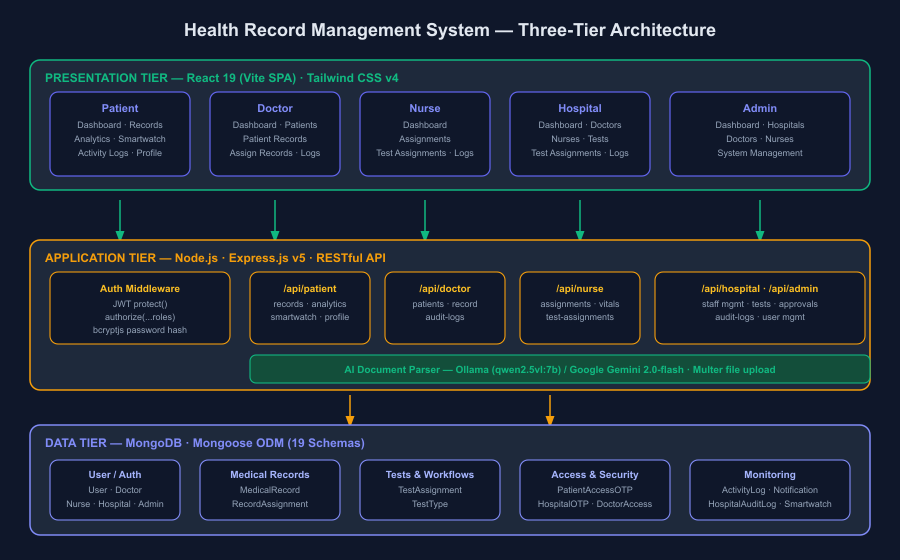
\includegraphics[width=\linewidth]{fig1_system_architecture}
\caption{Three-Tier Architecture of the Health Record Management System}
\label{fig:architecture}
\end{figure}

\subsection{3.1.2 User Authentication Flow}

Figure \ref{fig:auth_flow} illustrates the authentication and authorisation flow.

\begin{figure}[H]
\centering
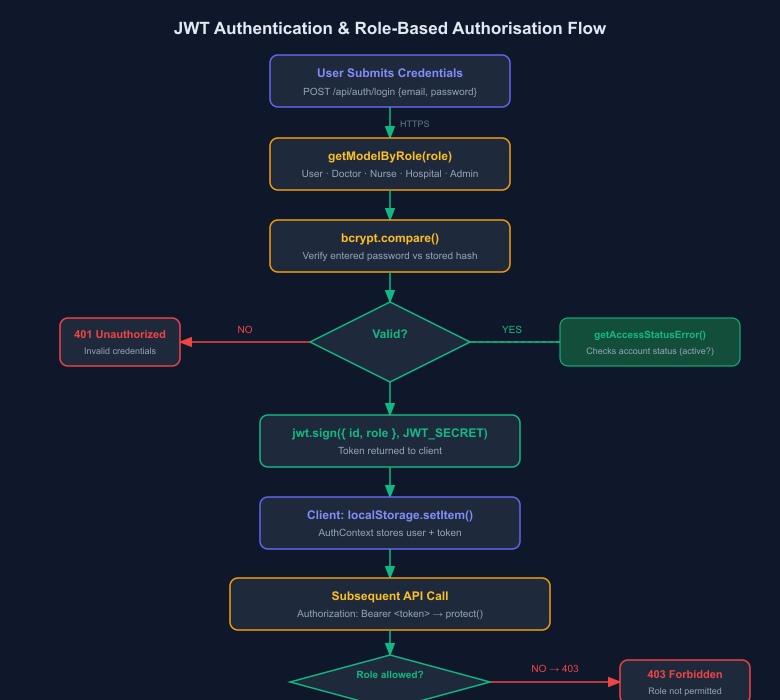
\includegraphics[width=0.72\linewidth]{fig2_auth_flow}
\caption{JWT Authentication and Role-Based Authorisation Flow}
\label{fig:auth_flow}
\end{figure}

The flow is as follows:
\begin{enumerate}
    \item User submits credentials (email + password) via the Login page.
    \item The backend verifies credentials against the appropriate role model (User, Doctor, Nurse, Hospital, or Admin) and compares the bcrypt hash.
    \item On success, a signed JWT (containing user ID and role) is returned.
    \item The React frontend stores the token in \texttt{localStorage} and attaches it as a Bearer token to all subsequent API requests.
    \item The \texttt{protect} middleware on the backend verifies the JWT signature and fetches the live user record. The \texttt{authorize(...roles)} middleware then checks role eligibility.
\end{enumerate}

\subsection{3.1.3 Medical Record Lifecycle}

\begin{figure}[H]
\centering
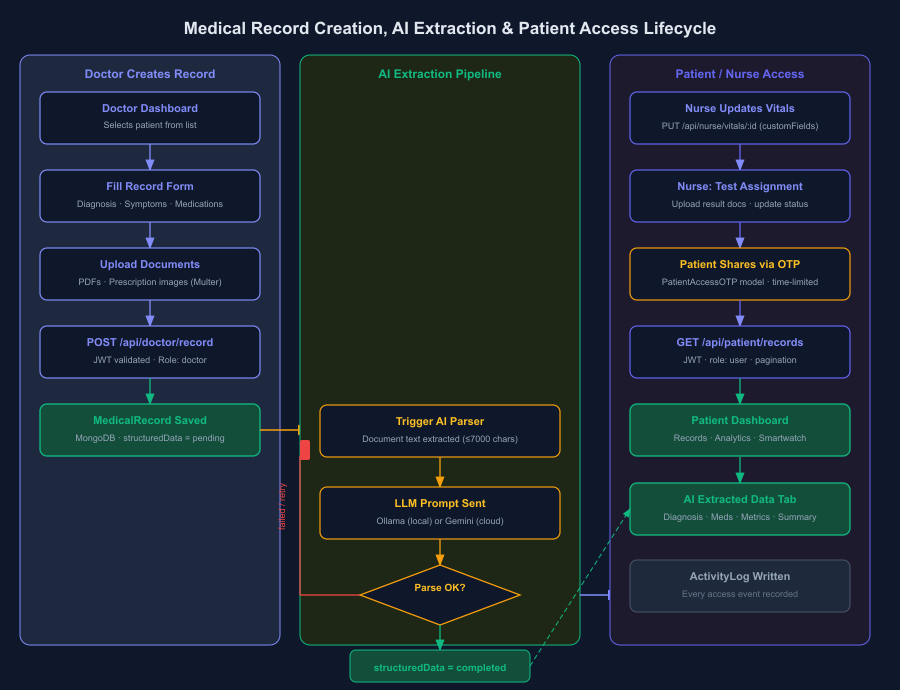
\includegraphics[width=\linewidth]{fig3_record_lifecycle}
\caption{Medical Record Creation, AI Extraction, and Patient Access Lifecycle}
\label{fig:record_lifecycle}
\end{figure}

\section{Algorithms and Techniques}

\subsection{3.2.1 Password Security}
Passwords are hashed using \texttt{bcryptjs} with a salt factor of 10 before storage. On login, the entered password is compared using \texttt{bcrypt.compare()}, which is resistant to timing attacks.

\subsection{3.2.2 JWT Authentication}
Authentication tokens are signed using the \texttt{jsonwebtoken} library with a server-side secret. The token payload carries the user ID and role, enabling the backend to route requests to the correct Mongoose model without an additional lookup step.

\subsection{3.2.3 AI Document Extraction Pipeline}
Uploaded medical PDFs are processed via a configurable AI provider:
\begin{enumerate}
    \item The file is stored in \texttt{/uploads/} using Multer.
    \item Text content is sent (up to 7,000 characters) to the configured provider (Ollama local LLM or Google Gemini API).
    \item The provider returns a JSON response containing: \texttt{diagnosis}, \texttt{specialization}, \texttt{medications}, \texttt{normalizedFields}, \texttt{numericFields}, \texttt{reportDate}, and \texttt{nextVisitDate}.
    \item The extracted data is stored in the \texttt{structuredData} sub-document of the \texttt{MedicalRecord} model.
    \item Validation errors and conflicts with existing values are tracked in dedicated array fields.
\end{enumerate}

\subsection{3.2.4 Role-Based Access Control (RBAC)}
Every backend route file begins with \texttt{protect} (JWT validation) and \texttt{authorize(...roles)} (role check) middleware. Frontend routes are guarded by a \texttt{ProtectedRoute} component that reads the authenticated user's role from the \texttt{AuthContext} and redirects unauthorised access to \texttt{/unauthorized}.

\subsection{3.2.5 OTP-Based Patient Record Sharing}
When a patient grants a hospital access to their records, a time-limited OTP is generated and stored in the \texttt{PatientAccessOTP} model. The hospital enters the OTP to obtain a temporary access grant, preventing unauthorised record viewing.

\section{Detailed Methodologies}

\subsection{3.3.1 Frontend Development Methodology}

The frontend follows a component-based architecture using React 19 with React Router DOM v7 for client-side routing. The design system implements the \textit{Governance Terminal} design language characterised by:

\begin{itemize}
    \item Dark mode with \texttt{slate-900} background and emerald (\texttt{\#10B981}) accent colour
    \item Glassmorphism card effects with \texttt{backdrop-filter: blur}
    \item Smooth CSS transitions and micro-animations (hover lifts, fade-ins)
    \item Responsive layouts using Tailwind CSS grid and flex utilities
    \item Inter / Space Grotesk typography via Google Fonts
\end{itemize}

The \texttt{ThemeProvider} context manages light/dark theme state globally. The \texttt{AccessibilityProvider} context persists accessibility preferences (text size, keyboard mode, dyslexia mode, etc.) both in memory and via API sync to the user's profile.

\subsection{3.3.2 Backend Development Methodology}

The backend follows RESTful API design conventions with resource-based URL structures:

\begin{itemize}
    \item \texttt{GET /api/patient/records} — fetch authenticated patient's records
    \item \texttt{POST /api/doctor/record} — create a new medical record (Doctor only)
    \item \texttt{PUT /api/nurse/record/:id} — update vitals on a record (Nurse only)
    \item \texttt{GET /api/hospital/doctors} — list affiliated doctors (Hospital only)
    \item \texttt{GET /api/admin/hospitals} — list all hospitals (Admin only)
\end{itemize}

Route files apply \texttt{protect} + \texttt{authorize} middleware internally, so the router only needs to define the endpoint logic.

\subsection{3.3.3 Database Design Methodology}

MongoDB was chosen for its flexible document model, which is well-suited to the heterogeneous nature of medical records (different hospitals use different fields). Mongoose schemas enforce data validation, default values, and indexing. Key indexes include:
\begin{itemize}
    \item \texttt{patient + createdAt} (descending) on \texttt{MedicalRecord} for pagination
    \item \texttt{patient + hospital} on \texttt{MedicalRecord} for hospital-scoped views
    \item Unique index on \texttt{SmartwatchConnection.patient}
\end{itemize}

\subsection{3.3.4 Accessibility Implementation Methodology}

WCAG 2.1 AA compliance was pursued through the \texttt{AccessibilityTools} component — a slide-out panel available on all authenticated pages. The panel exposes six toggles:

\begin{table}[H]
\centering
\caption{Table 3.1: Accessibility Features and Their HCI Rationale}
\begin{tabular}{p{3.5cm}p{4cm}p{5cm}}
\toprule
\textbf{Feature} & \textbf{CSS/DOM Effect} & \textbf{HCI Rationale} \\
\midrule
Text Size Scaling & Increases \texttt{font-size} root variable & Aids low-vision users \\
Keyboard Mode & Focus outlines made prominent & Motor impairment, screen reader support \\
Dyslexia Mode & Switches to OpenDyslexic font & Reduces letter confusion \\
Target Boost & Increases tap/ click target size & Aids users with tremors or motor issues \\
Form Assist Mode & Labels always visible above fields & Reduces cognitive load \\
Accessible Charts & Renders data as tables alongside bar charts & Screen reader accessibility \\
\bottomrule
\end{tabular}
\end{table}

% ============================================================
%  CHAPTER 4 — WORK DONE
% ============================================================
\chapter{Work Done}

\section{Implementation}

\subsection{4.1.1 Technology Stack}

\begin{table}[H]
\centering
\caption{Table 4.1: Technology Stack of the HRMS}
\begin{tabular}{lll}
\toprule
\textbf{Layer} & \textbf{Technology} & \textbf{Version} \\
\midrule
Frontend Build Tool & Vite & v7.3.1 \\
UI Library & React & v19.2.0 \\
Routing & React Router DOM & v7.13.1 \\
HTTP Client & Axios & v1.13.6 \\
CSS Framework & Tailwind CSS & v4.2.1 \\
Backend Runtime & Node.js & v18+ \\
Web Framework & Express.js & v5.2.1 \\
Database & MongoDB & v7+ \\
ODM & Mongoose & v9.2.4 \\
Authentication & JSON Web Token (JWT) & v9.0.3 \\
Password Hashing & bcryptjs & v3.0.3 \\
AI Provider (local) & Ollama (qwen2.5vl:7b) & -- \\
AI Provider (cloud) & Google Gemini & 2.0-flash \\
\bottomrule
\end{tabular}
\end{table}

\subsection{4.1.2 Database Models}

The system defines 19 Mongoose models. The primary models are summarised in Table 4.2.

\begin{table}[H]
\centering
\caption{Table 4.2: Primary Database Models}
\begin{tabular}{p{3.5cm}p{9cm}}
\toprule
\textbf{Model} & \textbf{Key Fields} \\
\midrule
\texttt{User} & \texttt{patientId}, \texttt{name}, \texttt{email}, \texttt{role}, \texttt{bloodGroup}, \texttt{medicalRecords[]}, \texttt{emergencyContact}, \texttt{accessibilityProfile} \\
\texttt{Doctor} & \texttt{specialization}, \texttt{qualifications[]}, \texttt{experience}, \texttt{consultationFee}, \texttt{hospitalAffiliation[]} \\
\texttt{Nurse} & \texttt{department}, \texttt{shift} (Morning/Evening/Night), \texttt{assignedPatients[]}, \texttt{qualifications[]} \\
\texttt{Hospital} & \texttt{registrationNumber}, \texttt{hospitalType}, \texttt{departments[]}, \texttt{facilities[]}, \texttt{totalBeds}, \texttt{accountStatus} \\
\texttt{Admin} & \texttt{adminLevel} (Admin/SuperAdmin/Moderator), \texttt{permissions[]}, \texttt{activityLog[]} \\
\texttt{MedicalRecord} & \texttt{patient}, \texttt{doctor}, \texttt{nurse}, \texttt{hospital}, \texttt{diagnosis}, \texttt{medications[]}, \texttt{healthMetrics}, \texttt{categorizedDocuments[]}, \texttt{structuredData}, \texttt{editHistory[]} \\
\texttt{SmartwatchConnection} & \texttt{provider}, \texttt{deviceId}, \texttt{latestMetrics} (heartRate, steps, calories, SpO\textsubscript{2}, sleepHours), \texttt{metricsHistory[]} \\
\texttt{TestAssignment} & \texttt{testType}, \texttt{assignedTo} (nurse), \texttt{status}, \texttt{resultDocuments[]} \\
\bottomrule
\end{tabular}
\end{table}

\subsection{4.1.3 Frontend Module Overview}

The application comprises 30+ page components organised by role. The route structure is as follows:

\begin{table}[H]
\centering
\caption{Table 4.3: Frontend Route Structure}
\begin{tabular}{lll}
\toprule
\textbf{Role} & \textbf{Routes} & \textbf{Key Pages} \\
\midrule
Patient & \texttt{/patient/*} & Dashboard, Profile, Medical Records, Health Analytics, Activity Logs, Smartwatch Insights \\
Doctor & \texttt{/doctor/*} & Dashboard, Patients, Patient Records, Assign Records, Audit Logs \\
Nurse & \texttt{/nurse/*} & Dashboard, Assignments, Test Assignments, Audit Logs \\
Hospital & \texttt{/hospital/*} & Dashboard, Doctors, Nurses, Tests, Test Assignments, Audit Logs \\
Admin & \texttt{/admin/*} & Dashboard, Hospitals, Doctors, Nurses \\
\bottomrule
\end{tabular}
\end{table}

\subsection{4.1.4 Key Feature Implementations}

\textbf{Patient Medical Records Module:}
The \texttt{PatientMedicalRecords} page is one of the most complex components, at approximately 1,500 lines of JSX. It supports:
\begin{itemize}
    \item Paginated list view of all records with search and filter by hospital and date range
    \item Per-record expansion with tabs: Summary, Documents, Health Metrics, Medications, and AI Extracted Data
    \item Inline PDF viewer and image preview for uploaded documents
    \item Parsed metric badges colour-coded by status (low/normal/high)
    \item AI-generated document summaries rendered per uploaded file
\end{itemize}

\textbf{Health Analytics Module:}
The \texttt{PatientHealthAnalytics} page renders time-series charts for blood sugar, blood pressure (systolic/diastolic), heart rate, weight, and thyroid (TSH) drawn from all medical records. Each chart is rendered using SVG path interpolation and includes accessible table fallback mode.

\textbf{Smartwatch Insights Module:}
The \texttt{PatientSmartwatchInsights} page allows patients to configure a wearable connection (Apple Health, Google Fit, Fitbit, Garmin) and view the latest and historical metrics: heart rate, step count, calories burned, SpO\textsubscript{2}, and sleep hours. Metrics are displayed on animated dial cards.

\textbf{AI Document Parsing:}
When a doctor uploads a PDF prescription or diagnostic report, the backend triggers the AI extraction pipeline. The provider reads the document text, returns structured JSON, and populates the \texttt{structuredData} field of the \texttt{MedicalRecord}. The frontend surfaces this data under the ``AI Extracted Data'' tab.

\textbf{Context-Aware Voice Help Button:}
A floating \texttt{ContextVoiceHelpButton} component is present on all authenticated pages. It uses the Web Speech API (\texttt{SpeechSynthesis}) to read out the page name and a brief description of available actions — providing a voice-first navigation aid for visually impaired users.

\subsection{4.1.5 API Architecture}

The backend exposes five main route groups:

\begin{table}[H]
\centering
\caption{Table 4.4: Backend API Route Groups and Sample Endpoints}
\begin{tabular}{p{3cm}p{10cm}}
\toprule
\textbf{Route Group} & \textbf{Sample Endpoints} \\
\midrule
\texttt{/api/auth} & POST \texttt{/login}, POST \texttt{/register}, GET \texttt{/me} \\
\texttt{/api/patient} & GET \texttt{/records}, GET \texttt{/analytics}, GET \texttt{/smartwatch}, PUT \texttt{/profile} \\
\texttt{/api/doctor} & GET \texttt{/patients}, POST \texttt{/record}, PUT \texttt{/record/:id}, GET \texttt{/audit-logs} \\
\texttt{/api/nurse} & GET \texttt{/assignments}, PUT \texttt{/vitals/:id}, GET \texttt{/test-assignments} \\
\texttt{/api/hospital} & GET \texttt{/doctors}, POST \texttt{/tests}, GET \texttt{/test-assignments}, GET \texttt{/audit-logs} \\
\texttt{/api/admin} & GET \texttt{/hospitals}, PUT \texttt{/hospital/:id/approve}, GET \texttt{/doctors}, GET \texttt{/nurses} \\
\bottomrule
\end{tabular}
\end{table}

\section{Results and Analysis}

\subsection{4.2.1 Functional Outcomes}

The following functional requirements were implemented and verified:

\begin{table}[H]
\centering
\caption{Table 4.5: Functional Requirements and Implementation Status}
\begin{tabular}{p{7cm}cc}
\toprule
\textbf{Requirement} & \textbf{Priority} & \textbf{Status} \\
\midrule
User registration and login (all roles) & High & \checkmark Implemented \\
JWT authentication and role-based route protection & High & \checkmark Implemented \\
Patient medical record creation (Doctor) & High & \checkmark Implemented \\
Patient medical record viewing (Patient) & High & \checkmark Implemented \\
Document upload for prescriptions (PDF/images) & High & \checkmark Implemented \\
AI-based document structured extraction & Medium & \checkmark Implemented \\
Health analytics charts (blood sugar, BP, HR, weight) & Medium & \checkmark Implemented \\
Smartwatch integration (metrics fetch and display) & Medium & \checkmark Implemented \\
Accessibility toolkit (6 modes) & High & \checkmark Implemented \\
OTP-based patient record sharing & Medium & \checkmark Implemented \\
Hospital staff management (doctors and nurses) & High & \checkmark Implemented \\
Admin hospital approval workflow & High & \checkmark Implemented \\
Audit log trail (per role) & Medium & \checkmark Implemented \\
Responsive mobile layout & High & \checkmark Implemented \\
\bottomrule
\end{tabular}
\end{table}

\subsection{4.2.2 Screen Descriptions}

\begin{figure}[H]
\centering
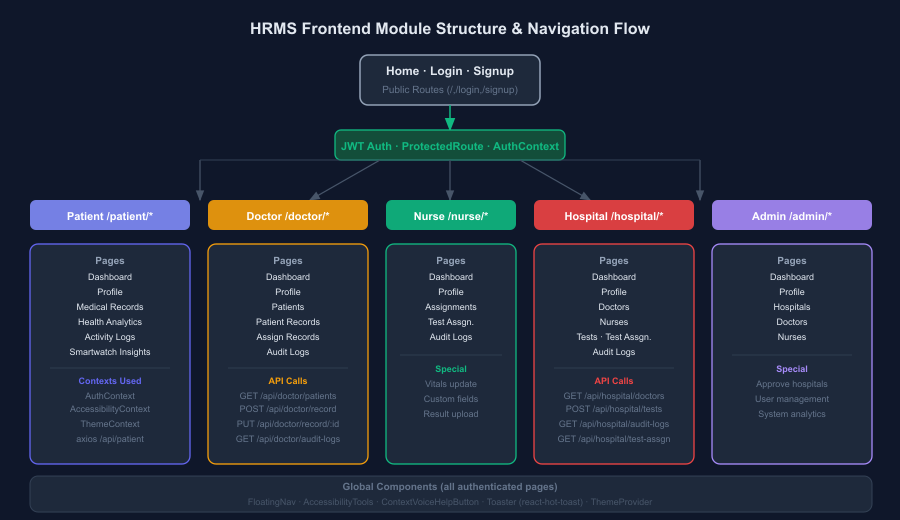
\includegraphics[width=\linewidth]{fig5_frontend_structure}
\caption{Patient Dashboard showing health summary, recent records, and smartwatch metrics}
\label{fig:patient_dashboard}
\end{figure}

\begin{figure}[H]
\centering
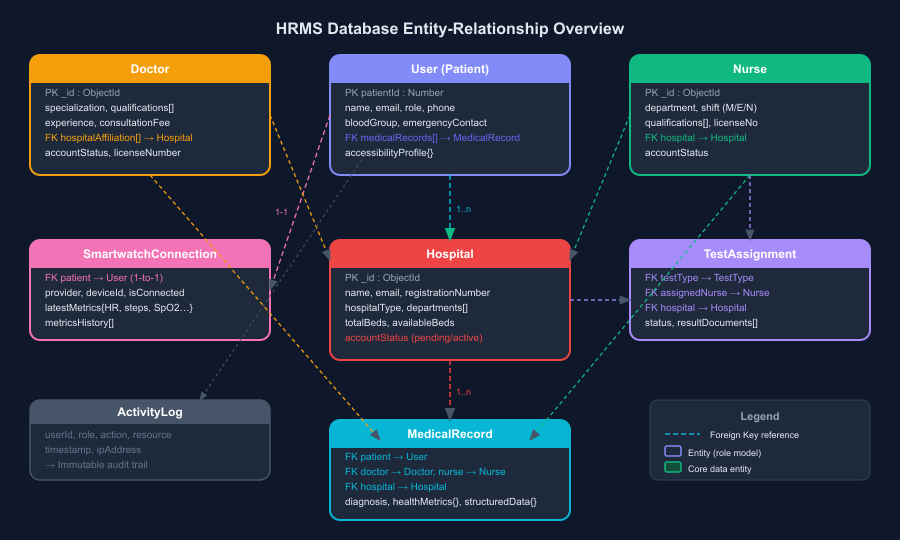
\includegraphics[width=\linewidth]{fig4_er_diagram}
\caption{Patient Medical Records page showing paginated record list with expanded detail view}
\label{fig:medical_records}
\end{figure}

\begin{figure}[H]
\centering
% Replace with actual screenshot: \includegraphics[width=\linewidth]{fig_doctor_dashboard}
\caption{Doctor Dashboard showing assigned patients and quick-action cards}
\label{fig:doctor_dashboard}
\end{figure}

\begin{figure}[H]
\centering
% Replace with actual screenshot: \includegraphics[width=\linewidth]{fig_accessibility_panel}
\caption{Accessibility Tools panel showing all six configurable modes}
\label{fig:accessibility_panel}
\end{figure}

\begin{figure}[H]
\centering
% Replace with actual screenshot: \includegraphics[width=\linewidth]{fig_health_analytics}
\caption{Health Analytics page showing time-series charts for key clinical metrics}
\label{fig:health_analytics}
\end{figure}

\subsection{4.2.3 HCI Evaluation}

The system was evaluated against Nielsen's 10 Usability Heuristics:

\begin{table}[H]
\centering
\caption{Table 4.6: Nielsen's Usability Heuristics Compliance}
\begin{tabular}{p{5.5cm}p{7cm}}
\toprule
\textbf{Heuristic} & \textbf{HRMS Implementation} \\
\midrule
Visibility of System Status & Toast notifications (react-hot-toast) for all async actions; loading spinners on data fetch \\
Match between System and Real World & Role-specific terminology (``Patient Records'' not ``User Documents'') \\
User Control and Freedom & Confirmation dialogs before destructive actions; cancel buttons on all modals \\
Consistency and Standards & Unified Governance Terminal design language across all 30+ pages \\
Error Prevention & Client-side form validation before API calls; file type restrictions on upload \\
Recognition over Recall & Sidebar navigation always visible; breadcrumbs on deep pages \\
Flexibility and Efficiency of Use & Keyboard navigation mode; search and filter on all list views \\
Aesthetic and Minimalist Design & Information density balanced with whitespace; card-based layouts \\
Help Users Recognise, Diagnose, and Recover from Errors & Descriptive error messages from backend surfaced in UI \\
Help and Documentation & Context Voice Help button reads page description aloud \\
\bottomrule
\end{tabular}
\end{table}

% ============================================================
%  CHAPTER 5 — CONCLUSION AND FUTURE WORK
% ============================================================
\chapter{Conclusion and Future Work}

The Health Record Management System presented in this report successfully demonstrates the application of Human--Computer Interaction principles to a real-world healthcare problem. By building a full-stack, multi-role web application centred on centralised patient records, the project achieves its primary objectives: reducing data fragmentation, enforcing role-based access control, integrating AI-assisted document parsing, and providing an accessible, responsive user interface.

From an HCI standpoint, the \textit{Governance Terminal} design language provides a consistent, high-quality visual experience across all five user roles. The comprehensive accessibility toolkit — featuring dyslexia mode, keyboard navigation, target boost, text scaling, form assist, and accessible charts — demonstrates that inclusive design can be elegantly integrated into a professional healthcare interface without sacrificing aesthetics or usability.

The integration of smartwatch data and AI-based document extraction positions HRMS as a platform aligned with next-generation healthcare trends: data-driven patient empowerment, longitudinal health monitoring, and intelligent clinical decision support.

\textbf{Limitations:} The current prototype does not implement a real FHIR-compliant API, and smartwatch integration relies on manual data entry through a custom API endpoint rather than direct OAuth integration with Apple Health or Google Fit. AI extraction accuracy is dependent on the quality of the uploaded document and the capabilities of the configured language model.

\textbf{Future Work:}
\begin{enumerate}
    \item \textbf{FHIR Compliance}: Implement HL7 FHIR R4 endpoints to enable interoperability with existing hospital information systems.
    \item \textbf{OAuth Wearable Integration}: Implement direct OAuth 2.0 flows with Apple HealthKit, Google Fit, and Fitbit APIs.
    \item \textbf{Telemedicine Module}: Add a video consultation feature using WebRTC, allowing patients to consult doctors within the platform.
    \item \textbf{Automated Notifications}: Push notifications for upcoming appointments, prescription reminders, and critical health metric alerts.
    \item \textbf{Offline Support}: Progressive Web App (PWA) capabilities for offline record viewing in low-connectivity settings.
    \item \textbf{Formal Usability Study}: Conduct a structured user study with real patients, doctors, and nurses using System Usability Scale (SUS) and task completion metrics.
    \item \textbf{AI Diagnostic Assistance}: Expand the AI pipeline to provide preliminary diagnostic suggestions based on aggregated health metrics.
\end{enumerate}

In conclusion, HRMS demonstrates that thoughtful HCI design — when applied to a domain as critical as healthcare — can produce systems that are simultaneously powerful, inclusive, and user-friendly.

% ============================================================
%  REFERENCES
% ============================================================
\chapter*{References}
\addcontentsline{toc}{chapter}{References}

\begingroup
\fontsize{10}{14}\selectfont
\setstretch{1.2}

\noindent[1] E.\ S.\ Berner, T.\ J.\ La Lande, ``Overview of Clinical Decision Support Systems,'' \textit{Clinical Decision Support Systems: Theory and Practice}, 2nd ed., Springer, New York, 2007.

\noindent[2] A.\ K.\ Jha, C.\ M.\ DesRoches, E.\ P.\ Campbell, K.\ Donelan, S.\ R.\ Rao, T.\ G.\ Ferris, A.\ Shields, S.\ Rosenbaum, and D.\ Blumenthal, ``Use of Electronic Health Records in U.S.\ Hospitals,'' \textit{New England Journal of Medicine}, vol.\ 360, no.\ 16, pp.\ 1628--1638, 2009.

\noindent[3] D.\ F.\ Ferraiolo, R.\ Sandhu, S.\ Gavrila, D.\ R.\ Kuhn, and R.\ Chandramouli, ``Proposed NIST Standard for Role-Based Access Control,'' \textit{ACM Transactions on Information and System Security}, vol.\ 4, no.\ 3, pp.\ 224--274, 2001.

\noindent[4] D.\ W.\ Roblin, T.\ K.\ Houston II, J.\ J.\ Allison, P.\ J.\ Joski, and E.\ Becker, ``Disparities in Use of a Personal Health Record in a Managed Care Organization,'' \textit{Journal of the American Medical Informatics Association}, vol.\ 16, no.\ 5, pp.\ 683--689, 2009.

\noindent[5] B.\ Middleton, M.\ Bloomrosen, M.\ A.\ Dente, B.\ Hashmat, R.\ Koppel, J.\ M.\ Overhage, T.\ H.\ Payne, S.\ T.\ Rosenbloom, C.\ Weaver, and J.\ Zhang, ``Enhancing Patient Safety and Quality of Care by Improving the Usability of Electronic Health Record Systems,'' \textit{Journal of the American Medical Informatics Association}, vol.\ 20, no.\ e1, pp.\ e2--e8, 2013.

\noindent[6] J.\ Lazar, D.\ Goldstein, and A.\ Taylor, \textit{Ensuring Digital Accessibility Through Process and Policy}, Morgan Kaufmann, Waltham, MA, 2015.

\noindent[7] P.\ Rajpurkar, E.\ Chen, O.\ Banerjee, and E.\ J.\ Topol, ``AI in Health and Medicine,'' \textit{Nature Medicine}, vol.\ 28, pp.\ 31--38, 2022.

\noindent[8] L.\ Piwek, D.\ A.\ Ellis, S.\ Andrews, and A.\ Joinson, ``The Rise of Consumer Health Wearables: Promises and Barriers,'' \textit{PLOS Medicine}, vol.\ 13, no.\ 2, e1001953, 2016.

\noindent[9] J.\ Nielsen, \textit{Usability Engineering}, Academic Press, New York, 1993.

\noindent[10] HL7 International, ``FHIR R4 Specification,'' Available at: \url{https://www.hl7.org/fhir/}; Last accessed on: April 14, 2026.

\noindent[11] React Documentation, Available at: \url{https://react.dev/}; Last accessed on: April 14, 2026.

\noindent[12] MongoDB Documentation, Available at: \url{https://www.mongodb.com/docs/}; Last accessed on: April 14, 2026.

\noindent[13] W3C, ``Web Content Accessibility Guidelines (WCAG) 2.1,'' Available at: \url{https://www.w3.org/TR/WCAG21/}; Last accessed on: April 14, 2026.

\noindent[14] Express.js Documentation, Available at: \url{https://expressjs.com/}; Last accessed on: April 14, 2026.

\endgroup

% ============================================================
%  APPENDIX
% ============================================================
\appendix
\chapter{Appendix}

\section{Acronyms}

\begin{table}[H]
\centering
\caption{Table A.1: Acronyms Used in This Report}
\begin{tabular}{ll}
\toprule
\textbf{Acronym} & \textbf{Full Form} \\
\midrule
EHR     & Electronic Health Record \\
HRMS    & Health Record Management System \\
HCI     & Human Computer Interaction \\
RBAC    & Role-Based Access Control \\
API     & Application Programming Interface \\
REST    & Representational State Transfer \\
JWT     & JSON Web Token \\
MERN    & MongoDB, Express, React, Node.js \\
SPA     & Single Page Application \\
OTP     & One-Time Password \\
AI      & Artificial Intelligence \\
LLM     & Large Language Model \\
FHIR    & Fast Healthcare Interoperability Resources \\
SpO\textsubscript{2}   & Peripheral Oxygen Saturation \\
TSH     & Thyroid Stimulating Hormone \\
WCAG    & Web Content Accessibility Guidelines \\
SUS     & System Usability Scale \\
PWA     & Progressive Web App \\
ODM     & Object Data Modeling \\
CORS    & Cross-Origin Resource Sharing \\
\bottomrule
\end{tabular}
\end{table}

\section{Project Repository Structure}

\begin{lstlisting}[language=bash, caption=Project Directory Structure]
Health-Record-Management-System/
├── backend/
│   ├── config/          # MongoDB connection
│   ├── middleware/       # JWT protect + authorize
│   ├── models/          # 19 Mongoose schemas
│   ├── routes/          # auth, patient, doctor, nurse, hospital, admin
│   ├── utils/           # Role helpers, AI provider
│   ├── scripts/         # Seed scripts
│   └── server.js        # Express app entry point
└── frontend/
    ├── src/
    │   ├── components/  # Reusable UI components
    │   ├── context/     # Auth, Theme, Accessibility contexts
    │   ├── pages/       # 30+ role-scoped page components
    │   ├── services/    # Axios API service wrappers
    │   ├── utils/       # Utility functions
    │   ├── App.jsx      # Root router
    │   └── index.css    # Global styles + design tokens
    └── index.html
\end{lstlisting}

\section{Environment Configuration Reference}

\begin{lstlisting}[language=bash, caption=Backend .env Configuration Variables]
PORT=5000
MONGODB_URI=mongodb://localhost:27017/health-record-system
JWT_SECRET=<your_secret_key>
NODE_ENV=development

# AI provider switch
AI_PROVIDER=local          # 'local' (Ollama) or 'gemini'
AI_FALLBACK_PROVIDER=local
AI_MAX_INPUT_CHARS=7000
AI_TIMEOUT_MS=300000

# Ollama config
OLLAMA_MODEL=qwen2.5vl:7b
OLLAMA_GENERATE_URL=http://localhost:11434/api/generate

# Gemini config
GEMINI_API_KEY=<your_gemini_key>
GEMINI_MODEL=gemini-2.0-flash
\end{lstlisting}

\end{document}
